Figure \ref{fig:first-mixture} on page \pageref{fig:first-mixture} shows a special kind of a proportional symbol map. According to figure \ref{fig:va-channels} on page \pageref{fig:va-channels}, this type of map uses the visual channel of size to represent differences of discrete data. Again, this type of map can be subdivided into two categories: classed and unclassed. Classed ones are known as range-graded or graduated symbol maps, whereas unclassed ones are called proportional symbol maps. The latter one uses a symbol size proportional to the value of the attribute being mapped \iacite{Dutton.2014}.
Although circles are the most typical symbol used, it is possible to use any type of symbol, ranging from abstract, geometric symbols to pictographic symbols. Figure \ref{fig:different-symbols} on page \pageref{fig:different-symbols} shows two proportional symbol maps showing the same phenomenon. The left part of this figure uses the common circle as symbol, while the right side uses a pictogram. Albeit the established circle because of their compactness due to their low perimeter to area ratio, \citeauthor{Dutton.2014} says, that squares or bars are easier to estimate the size of the symbol.

\begin{figure}[!htb]
\centering
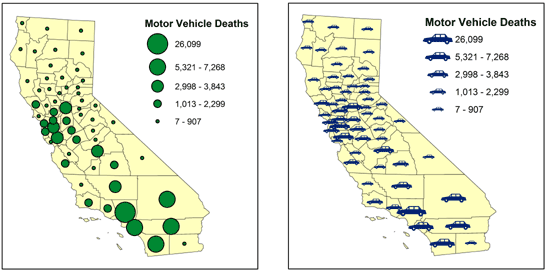
\includegraphics[height=5cm,keepaspectratio]{images/psm/symbols.png}
\caption[
    Two types of proportional symbol maps with different symbols \iacite{Dutton.2014}.
]{Two types of proportional symbol maps with different symbols.}
\label{fig:different-symbols}
\end{figure}

Another consideration in terms of symbol used is the fact, that squares and bars tend to run off the page with large values earlier than circles might \iacite{Dutton.2014}. \citeauthor{FLANNERY1971} introduced a scaling factor for proportional circles for better estimation of the value. However, this correction may not be very effective, because the correction itself does not consider the map context \iacite{FLANNERY1971}. A phenomenon related to the importance of context is known as the ebbinghaus illusion. Figure \ref{fig:ebbinghaus} on \pageref{fig:ebbinghaus} shows such an illusion. Both central circles actually have the same size, but because of the context of each side, the central circles appear different.

\begin{figure}[!htb]
\centering
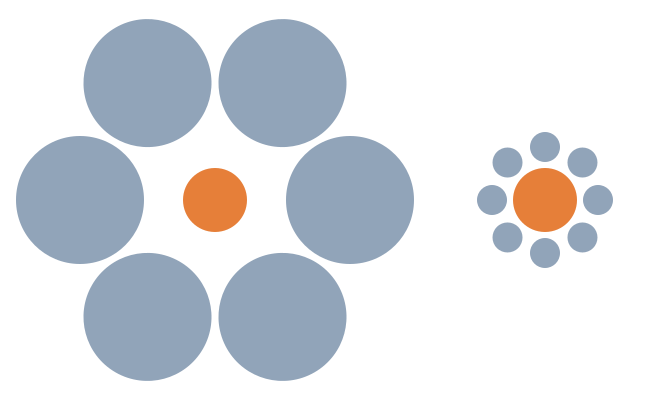
\includegraphics[height=5cm,keepaspectratio]{images/psm/ebbinghaus.png}
\caption[
    Ebbinghaus illusion, Urldate: 07.2016 \newline
    \small\texttt{\url{https://upload.wikimedia.org/wikipedia/commons/b/bc/Mond-vergleich.svg}}
]{Ebbinghaus illusion}
\label{fig:ebbinghaus}
\end{figure}

In order to combat the problem of value estimation, there are two major choices:
\begin{enumerate}
\item A legend could show proportional symbols which represent the different values of the mapped phenomenon. One possibility would be to display the smallest symbol, the largest symbol and some symbols at intermediate values.
\item Another alternative is to use range-graded symbols. Therefore the data needs to be classified, but in exchange the estimation problem is completly avoided. This alternative still needs consideration in the size of symbols, because each symbol should still be differentiable from each other.
\end{enumerate}

Based on the given knowledge about proportional and gradient symbol maps, it is possible to derive some main design principles:
\begin{itemize}
\item The estimation of the value of a symbol is key for this type of map. This is most easily accomplished with geometric symbols.
\item Use a legend with exmaples to increase the reader's ability to correctly estimate the value of a symbol.
\end{itemize}

A close related problem to the user's estimation problem is the actual scaling technique used. According to \citeauthor{Dent2008} the three most commong techniques used are
\begin{enumerate*}
\item absolute scaling,
\item apparent magnitude scaling and
\item range grading \iacite{Dent2008}.
\end{enumerate*}

\begin{enumerate}
\ditem{Absolute scaling} makes each symbol fit it's dat value on the scale being used. This means, that a symbol representing four items in a dataset is twice as big as a symbol representing two.
\ditem{Apparent magnitude scaling} compensates for human error interpretation in scale. Using this technique, a symbol having twice as much in value is not twice as big, because it would appear smaller, leading to interpretation error. This type of scaling takes this error into account and increased the size of a symbol by more than the proportional amount \iacite{Krygier.2007}.
\ditem{Range grading} classifies the data into a fixed amount of groups. Each group has a fixed range of values and the same symbol to represent. The groups only differ in the range of values they represent and the size of the symbols.
\end{enumerate}

The main advantage of a proportional symbol map is the flexibility it comes along with. Possible data can either be numerical or categorical nature. Even the way the data is used is adjustable. An item can be mapped on a precise location or to geographic areas, depending on the level of detail.
Comparing proportional symbol maps with dot density maps, one advantage is observable: the estimation problem of dot density maps becomes less tedious when using proportional symbols. However, if proportional symbol maps are put in comparison with choropleth maps, they also have an advantage: the size of the enumeration unit does not matter. This problem will be explained in detail in chapter \ref{s:choropleth} on page \pageref{s:choropleth}.